\chapter{System Design and Architecture}

\section{High-Level System Architecture}
The Thesis and Project Management System (TPMS) adopts a three-tier client-server architectural paradigm~\citep{martin2017clean} that enforces strict separation of concerns across presentation, business logic, and data persistence layers. Figure~\ref{fig:system_arch} depicts the high-level layered architecture.

\begin{figure}[H]
\centering
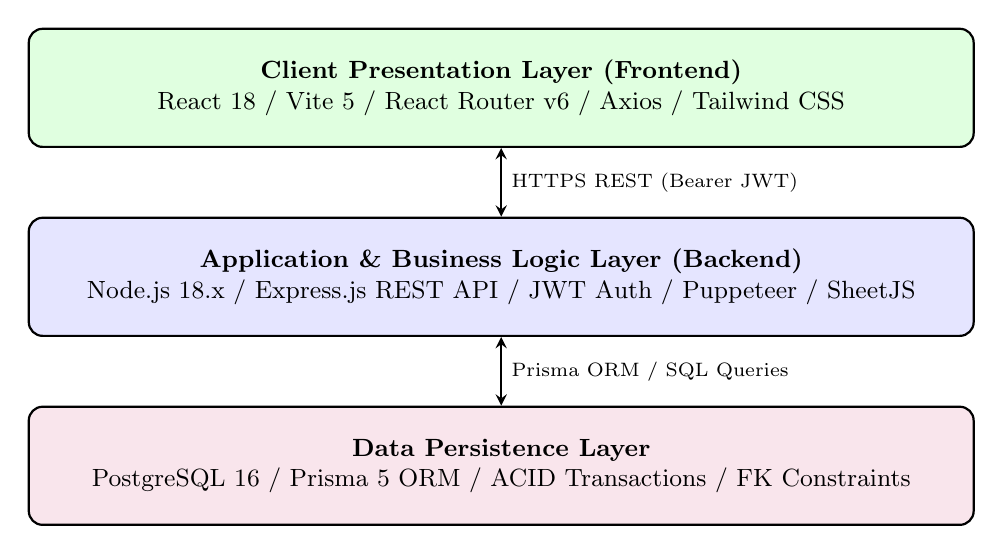
\begin{tikzpicture}[
    layer/.style={draw, thick, rounded corners=5pt, minimum width=12cm, minimum height=1.5cm,
                  align=center, font=\small},
    arr/.style={thick, <->, >=stealth, font=\scriptsize}
]
\node[layer, fill=green!12] (fe) at (0, 0)
    {\textbf{Client Presentation Layer (Frontend)}\\
     React 18 / Vite 5 / React Router v6 / Axios / Tailwind CSS};

\node[layer, fill=blue!10] (be) at (0,-2.4)
    {\textbf{Application \& Business Logic Layer (Backend)}\\
     Node.js 18.x / Express.js REST API / JWT Auth / Puppeteer / SheetJS};

\node[layer, fill=purple!10] (db) at (0,-4.8)
    {\textbf{Data Persistence Layer}\\
     PostgreSQL 16 / Prisma 5 ORM / ACID Transactions / FK Constraints};

\draw[arr] (fe) -- node[right, font=\scriptsize]{HTTPS REST (Bearer JWT)} (be);
\draw[arr] (be) -- node[right, font=\scriptsize]{Prisma ORM / SQL Queries} (db);
\end{tikzpicture}
\caption{Three-Tier System Architecture of TPMS}
\label{fig:system_arch}
\end{figure}

\begin{enumerate}
    \item \textbf{Client Presentation Layer:} A single-page application (SPA) built with React 18 and Vite 5, enforcing JWT-based route guards for five distinct role dashboards.
    \item \textbf{Application and Business Logic Layer:} Express.js RESTful API on Node.js encapsulating authentication, engagement guards, conflict-of-interest filters, and Puppeteer PDF rendering.
    \item \textbf{Data Persistence Layer:} PostgreSQL 16 managed via Prisma 5 ORM, providing ACID transactional integrity, compound indexes, and referential constraint enforcement across 14 relational tables.
\end{enumerate}

\section{Data Flow Diagrams (DFDs)}

\subsection{Context Diagram (Level 0)}
Figure~\ref{fig:dfd0} presents the Level 0 Context Diagram showing information flows between the five external stakeholders and the TPMS system.

\begin{figure}[H]
\centering
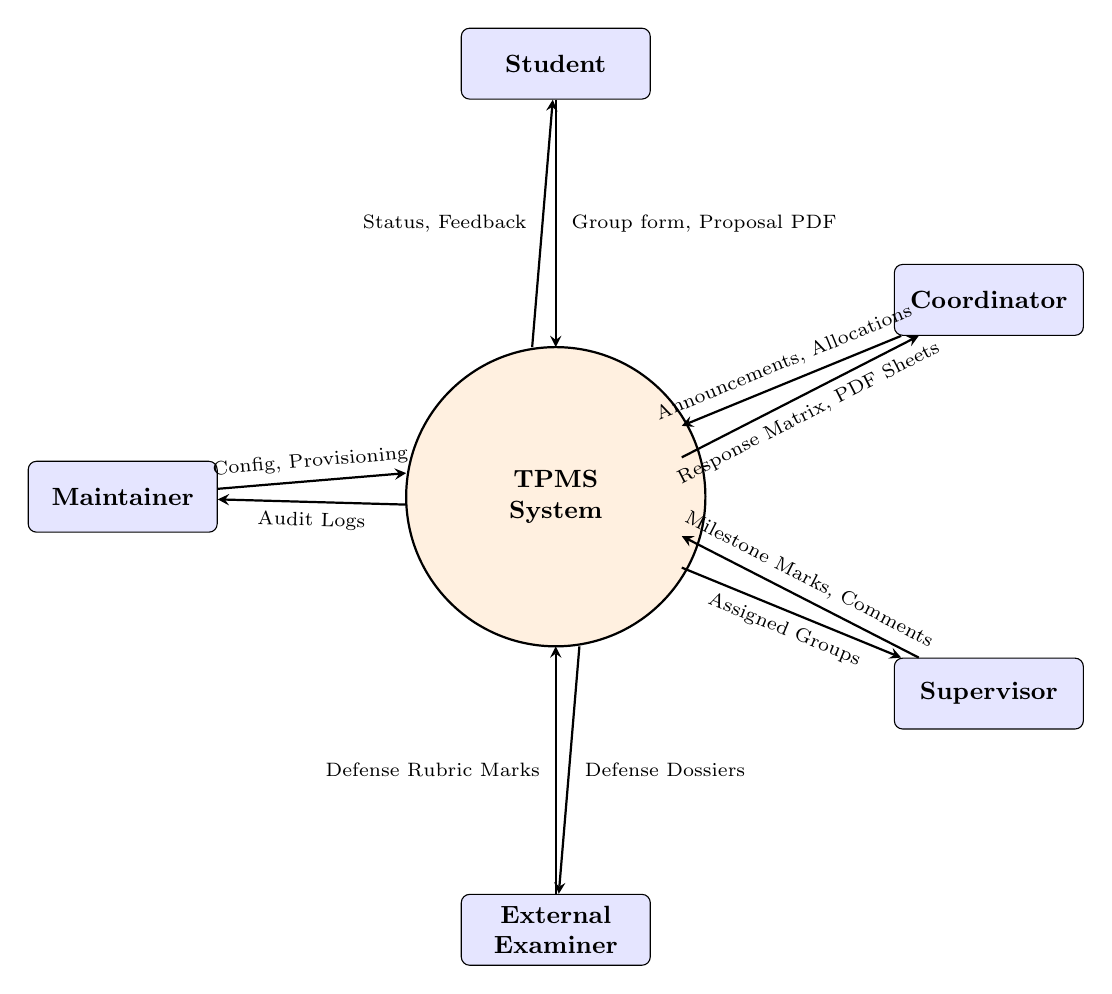
\begin{tikzpicture}[
    ent/.style={draw, fill=blue!10, rounded corners=3pt, minimum width=2.4cm,
                minimum height=0.9cm, align=center, font=\small\bfseries},
    sys/.style={draw, thick, fill=orange!12, circle, minimum size=3.8cm,
                align=center, font=\small\bfseries},
    arr/.style={->, >=stealth, thick, font=\scriptsize},
    rarr/.style={<-, >=stealth, thick, font=\scriptsize}
]
\node[sys] (sys) at (0,0) {TPMS\\System};

\node[ent] (student)   at ( 0,  5.5) {Student};
\node[ent] (coord)     at ( 5.5, 2.5) {Coordinator};
\node[ent] (super)     at ( 5.5,-2.5) {Supervisor};
\node[ent] (ext)       at ( 0, -5.5) {External\\Examiner};
\node[ent] (maint)     at (-5.5,  0) {Maintainer};

\draw[arr]  (student)  -- node[right, xshift=2pt]{\scriptsize Group form, Proposal PDF} (0, 1.9);
\draw[rarr] (student)  -- node[left,  xshift=-2pt]{\scriptsize Status, Feedback}         (-0.3, 1.9);

\draw[arr]  (coord) -- node[above, sloped]{\scriptsize Announcements, Allocations} (1.6, 0.9);
\draw[rarr] (coord) -- node[below, sloped]{\scriptsize Response Matrix, PDF Sheets} (1.6, 0.5);

\draw[arr]  (super) -- node[above, sloped]{\scriptsize Milestone Marks, Comments} (1.6,-0.5);
\draw[rarr] (super) -- node[below, sloped]{\scriptsize Assigned Groups}            (1.6,-0.9);

\draw[arr]  (ext) -- node[left, xshift=-2pt]{\scriptsize Defense Rubric Marks} (0,-1.9);
\draw[rarr] (ext) -- node[right,xshift=2pt]{\scriptsize Defense Dossiers}      (0.3,-1.9);

\draw[arr]  (maint) -- node[above, sloped]{\scriptsize Config, Provisioning} (-1.9, 0.3);
\draw[rarr] (maint) -- node[below, sloped]{\scriptsize Audit Logs}            (-1.9,-0.1);
\end{tikzpicture}
\caption{Level 0 Context Data Flow Diagram}
\label{fig:dfd0}
\end{figure}

\subsection{Level 1 Data Flow Diagram}
Figure~\ref{fig:dfd1} shows the Level 1 DFD decomposing TPMS into its six primary functional sub-processes.

\begin{figure}[H]
\centering
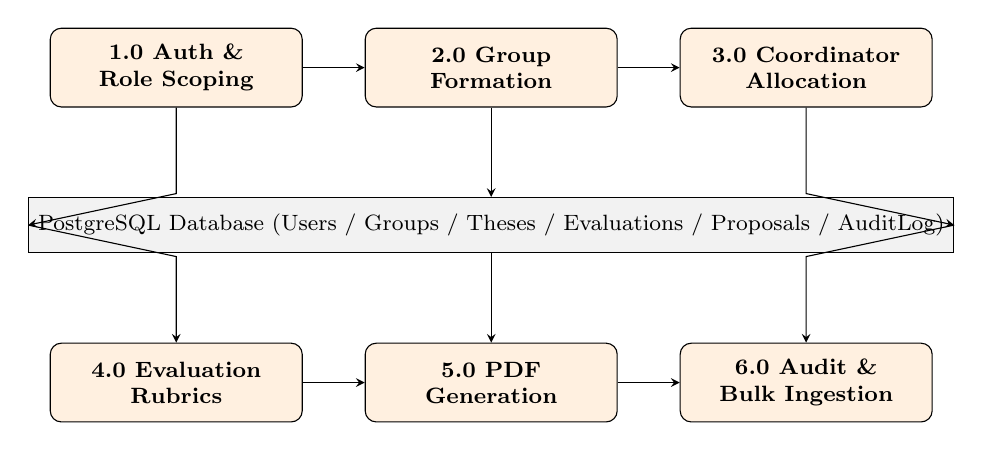
\begin{tikzpicture}[
    proc/.style={draw, fill=orange!12, rounded corners=4pt, minimum width=3.2cm,
                 minimum height=1.0cm, align=center, font=\footnotesize\bfseries},
    store/.style={draw, fill=gray!10, minimum width=9cm, minimum height=0.7cm,
                  align=center, font=\footnotesize},
    arr/.style={->, >=stealth, font=\scriptsize}
]
\node[proc] (p1) at (-5.5, 4) {1.0 Auth \&\\Role Scoping};
\node[proc] (p2) at (-1.5, 4) {2.0 Group\\Formation};
\node[proc] (p3) at ( 2.5, 4) {3.0 Coordinator\\Allocation};
\node[proc] (p4) at (-5.5, 0) {4.0 Evaluation\\Rubrics};
\node[proc] (p5) at (-1.5, 0) {5.0 PDF\\Generation};
\node[proc] (p6) at ( 2.5, 0) {6.0 Audit \&\\Bulk Ingestion};

\node[store] (db) at (-1.5, 2) {PostgreSQL Database (Users / Groups / Theses / Evaluations / Proposals / AuditLog)};

\draw[arr] (p1) -- (p2);
\draw[arr] (p2) -- (p3);
\draw[arr] (p4) -- (p5);
\draw[arr] (p5) -- (p6);
\draw[arr] (p1.south) -- (-5.5,2.4) -- (db.west);
\draw[arr] (db.west)  -- (-5.5,1.6) -- (p4.north);
\draw[arr] (p2.south) -- (-1.5,2.4) -- (db);
\draw[arr] (db)       -- (-1.5,1.6) -- (p5.north);
\draw[arr] (p3.south) -- ( 2.5,2.4) -- (db.east);
\draw[arr] (db.east)  -- ( 2.5,1.6) -- (p6.north);
\end{tikzpicture}
\caption{Level 1 Data Flow Diagram}
\label{fig:dfd1}
\end{figure}

\section{Use Case Diagram}
Figure~\ref{fig:usecase} illustrates the system use cases distributed across the five actor roles.

\begin{figure}[H]
\centering
\begin{tikzpicture}[
    actor/.style={draw, fill=green!10, rounded corners=3pt, minimum width=2.3cm,
                  minimum height=0.85cm, align=center, font=\footnotesize\bfseries},
    uc/.style={draw, ellipse, fill=blue!8, minimum width=4.2cm, minimum height=0.7cm,
               align=center, font=\scriptsize},
    line/.style={-}
]
\node[actor] (student)  at (-5.5,  5.5) {Student};
\node[actor] (super)    at (-5.5,  2.5) {Supervisor};
\node[actor] (coord)    at (-5.5, -0.5) {Coordinator};
\node[actor] (ext)      at (-5.5, -3.0) {Ext.~Examiner};
\node[actor] (maint)    at (-5.5, -5.0) {Maintainer};

\node[uc] (uc1) at (2.0,  6.8) {Form Group / Send Invitations};
\node[uc] (uc2) at (2.0,  5.7) {Upload Proposal and Reports};
\node[uc] (uc3) at (2.0,  4.6) {Track Evaluation Status};
\node[uc] (uc4) at (2.0,  3.3) {Review Proposals and Feedback};
\node[uc] (uc5) at (2.0,  2.2) {Submit Milestone Marks};
\node[uc] (uc6) at (2.0,  0.9) {Publish Announcements};
\node[uc] (uc7) at (2.0, -0.2) {Assign Supervisor and Examiner};
\node[uc] (uc8) at (2.0, -1.3) {Generate PDF Grade Sheets};
\node[uc] (uc9) at (2.0, -3.0) {Submit Defense Rubric Marks};
\node[uc] (uc10) at (2.0,-5.0) {Bulk Import and System Config};

\draw[dashed, rounded corners=6pt] (-0.2,-5.6) rectangle (6.5,7.4);
\node[font=\scriptsize, gray] at (3.0, 7.1) {TPMS System Boundary};

\draw[line] (student) -- (uc1);
\draw[line] (student) -- (uc2);
\draw[line] (student) -- (uc3);
\draw[line] (super)   -- (uc4);
\draw[line] (super)   -- (uc5);
\draw[line] (coord)   -- (uc6);
\draw[line] (coord)   -- (uc7);
\draw[line] (coord)   -- (uc8);
\draw[line] (ext)     -- (uc9);
\draw[line] (maint)   -- (uc10);
\end{tikzpicture}
\caption{System Use Case Diagram}
\label{fig:usecase}
\end{figure}

\section{Activity Diagram: Group Formation and Proposal Lifecycle}
Figure~\ref{fig:activity} shows the activity flow from team formation through coordinator finalization and rubric generation.

\begin{figure}[H]
\centering
\begin{tikzpicture}[
    start/.style={circle, fill=black, minimum size=0.5cm},
    stop/.style={circle, fill=black, minimum size=0.5cm, double, double distance=2pt},
    act/.style={draw, rounded corners=4pt, fill=blue!8, minimum width=8.5cm,
                minimum height=0.8cm, align=center, font=\footnotesize},
    dec/.style={draw, diamond, fill=yellow!18, minimum width=3.0cm,
                align=center, font=\scriptsize, aspect=2.5},
    arr/.style={->, >=stealth, font=\scriptsize}
]
\node[start]  (s)   at (0, 13)  {};
\node[act]    (a1)  at (0, 11.8) {Student initiates Project Group from active Announcement};
\node[act]    (a2)  at (0, 10.7) {Search peers by Roll Number or Name};
\node[act]    (a3)  at (0,  9.6) {Dispatch Invitation to peer students};
\node[dec]    (d1)  at (0,  8.2) {All peers\\accepted?};
\node[act]    (a4)  at (0,  6.9) {Upload compulsory Proposal PDF document};
\node[act]    (a5)  at (0,  5.8) {Submit Group to Coordinator Response Matrix};
\node[act]    (a6)  at (0,  4.7) {Coordinator: Fuzzy match supervisor and Finalize};
\node[act]    (a7)  at (0,  3.6) {System auto-generates Evaluation Rubric Components};
\node[stop]   (e)   at (0,  2.5) {};

\draw[arr] (s)  -- (a1);
\draw[arr] (a1) -- (a2);
\draw[arr] (a2) -- (a3);
\draw[arr] (a3) -- (d1);
\draw[arr] (d1) -- node[right]{\scriptsize Yes} (a4);
\draw[arr] (d1.east) -- ++(2.5,0) |- node[near end, right]{\scriptsize No (Pending)} (a3.east);
\draw[arr] (a4) -- (a5);
\draw[arr] (a5) -- (a6);
\draw[arr] (a6) -- (a7);
\draw[arr] (a7) -- (e);
\end{tikzpicture}
\caption{Activity Diagram: Group Formation and Proposal Submission Lifecycle}
\label{fig:activity}
\end{figure}

\section{Database Entity-Relationship Diagram}
Figure~\ref{fig:er} shows the simplified entity-relationship diagram of the TPMS core database tables.

\begin{figure}[H]
\centering
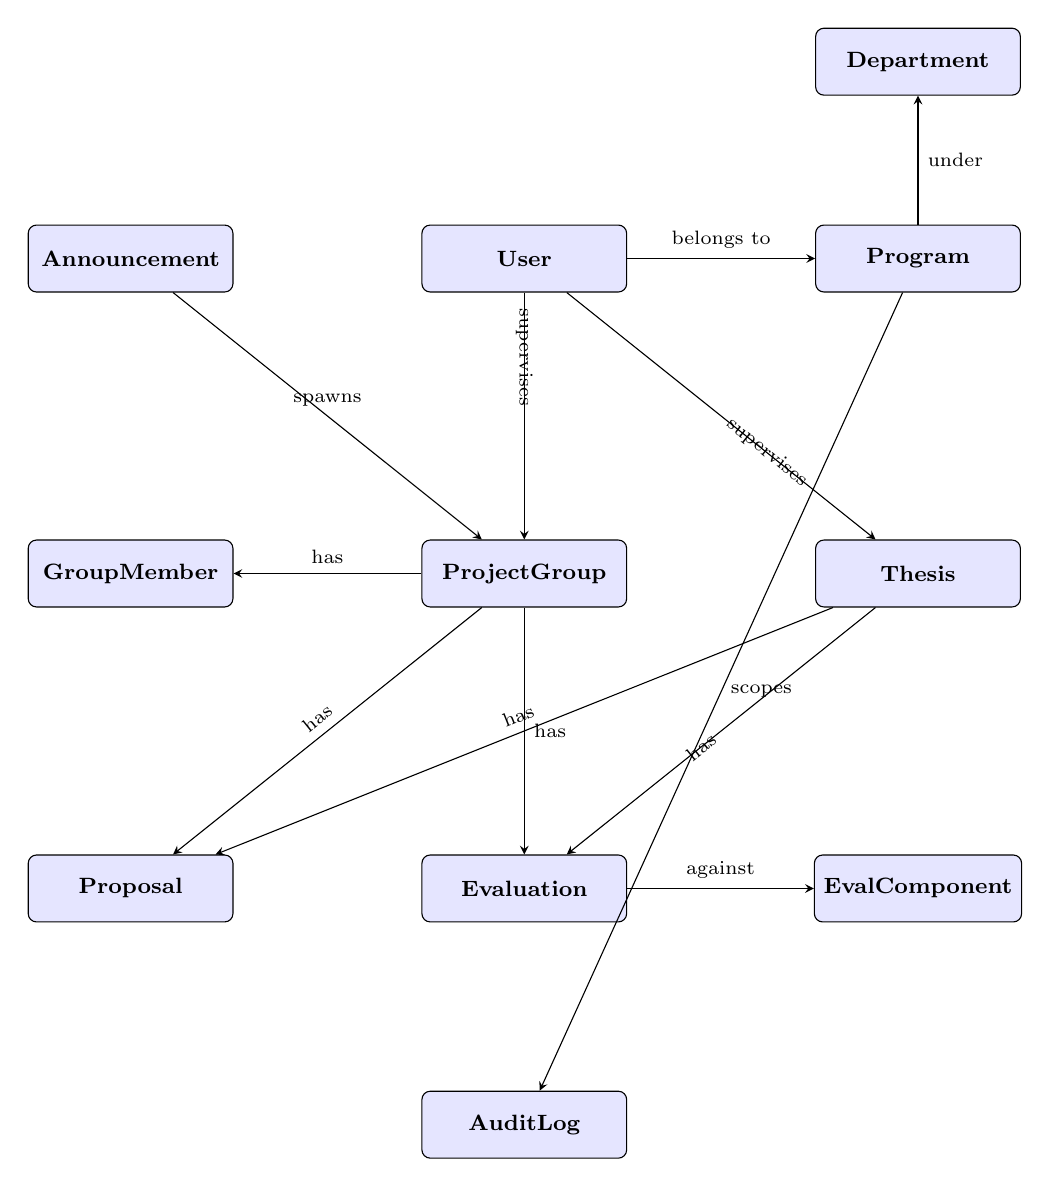
\begin{tikzpicture}[
    ent/.style={draw, fill=blue!10, rounded corners=3pt, minimum width=2.6cm,
                minimum height=0.85cm, align=center, font=\footnotesize\bfseries},
    arr/.style={->, >=stealth, font=\scriptsize}
]
\node[ent] (user)      at ( 0,  6)  {User};
\node[ent] (prog)      at ( 5,  6)  {Program};
\node[ent] (dept)      at ( 5,  8.5) {Department};
\node[ent] (ann)       at (-5,  6)  {Announcement};
\node[ent] (group)     at ( 0,  2)  {ProjectGroup};
\node[ent] (member)    at (-5,  2)  {GroupMember};
\node[ent] (thesis)    at ( 5,  2)  {Thesis};
\node[ent] (eval)      at ( 0, -2)  {Evaluation};
\node[ent] (comp)      at ( 5, -2)  {EvalComponent};
\node[ent] (proposal)  at (-5, -2)  {Proposal};
\node[ent] (audit)     at ( 0, -5)  {AuditLog};

\draw[arr] (user)    -- node[above]{\scriptsize belongs to}  (prog);
\draw[arr] (prog)    -- node[right]{\scriptsize under}       (dept);
\draw[arr] (user)    -- node[left, sloped]{\scriptsize supervises} (group);
\draw[arr] (ann)     -- node[above]{\scriptsize spawns}      (group);
\draw[arr] (group)   -- node[above]{\scriptsize has}         (member);
\draw[arr] (group)   -- node[right]{\scriptsize has}         (eval);
\draw[arr] (thesis)  -- node[left, sloped]{\scriptsize has}  (eval);
\draw[arr] (eval)    -- node[above]{\scriptsize against}     (comp);
\draw[arr] (group)   -- node[above, sloped]{\scriptsize has} (proposal);
\draw[arr] (thesis)  -- node[above, sloped]{\scriptsize has} (proposal);
\draw[arr] (prog)    -- node[right]{\scriptsize scopes}      (audit);
\draw[arr] (user)    -- node[right, sloped]{\scriptsize supervises} (thesis);
\end{tikzpicture}
\caption{Simplified Entity-Relationship Diagram of TPMS Database}
\label{fig:er}
\end{figure}

\section{Database Design}

\subsection{Data Dictionary}

\begin{table}[H]
\centering
\footnotesize
\caption{Data Dictionary: \texttt{User} Table}
\label{tab:schema_user}
\vspace{4pt}
\begin{tabularx}{\textwidth}{|l|l|l|X|}
\hline
\textbf{Field} & \textbf{Type} & \textbf{Constraint} & \textbf{Description} \\
\hline
\texttt{id} & \texttt{SERIAL} & \texttt{PK} & Auto-incrementing user identifier. \\
\texttt{email} & \texttt{VARCHAR} & \texttt{UNIQUE, NN} & Institutional email (\texttt{@pcampus.edu.np}). \\
\texttt{password} & \texttt{VARCHAR} & \texttt{NN} & bcrypt hashed password (work factor 10). \\
\texttt{role} & \texttt{ENUM} & \texttt{NN} & MAINTAINER, COORDINATOR, SUPERVISOR, STUDENT, EXTERNAL\_EXAMINER. \\
\texttt{degreeType} & \texttt{ENUM} & Nullable & BACHELOR or MASTER. \\
\texttt{canSupervise} & \texttt{BOOLEAN} & Default: false & Faculty supervision eligibility flag. \\
\texttt{rollNumber} & \texttt{VARCHAR} & Nullable & Student roll number (e.g., PUL080BCT084). \\
\texttt{programId} & \texttt{INTEGER} & \texttt{FK} & References student or coordinator program. \\
\hline
\end{tabularx}
\end{table}

\begin{table}[H]
\centering
\footnotesize
\caption{Data Dictionary: \texttt{ProjectGroup} Table}
\label{tab:schema_group}
\vspace{4pt}
\begin{tabularx}{\textwidth}{|l|l|l|X|}
\hline
\textbf{Field} & \textbf{Type} & \textbf{Constraint} & \textbf{Description} \\
\hline
\texttt{id} & \texttt{SERIAL} & \texttt{PK} & Unique group identifier. \\
\texttt{projectTitle} & \texttt{VARCHAR} & \texttt{NN} & Full title of the Bachelor project. \\
\texttt{projectType} & \texttt{ENUM} & Default: MINOR & MINOR or MAJOR. \\
\texttt{cluster} & \texttt{VARCHAR} & Nullable & Research cluster (EII, AIML, IPCV, etc.). \\
\texttt{status} & \texttt{ENUM} & Default: PENDING & PENDING, ACTIVE, COMPLETED, OVERDUE, REJECTED. \\
\texttt{supervisorId} & \texttt{INTEGER} & \texttt{FK} & References assigned supervisor in User table. \\
\texttt{programId} & \texttt{INTEGER} & \texttt{FK} & References owning academic program. \\
\texttt{academicYearId} & \texttt{INTEGER} & \texttt{FK} & References active academic semester. \\
\hline
\end{tabularx}
\end{table}

\begin{table}[H]
\centering
\footnotesize
\caption{Data Dictionary: \texttt{Evaluation} Table}
\label{tab:schema_eval}
\vspace{4pt}
\begin{tabularx}{\textwidth}{|l|l|l|X|}
\hline
\textbf{Field} & \textbf{Type} & \textbf{Constraint} & \textbf{Description} \\
\hline
\texttt{id} & \texttt{SERIAL} & \texttt{PK} & Unique evaluation record. \\
\texttt{componentId} & \texttt{INTEGER} & \texttt{FK} & References rubric sub-criterion. \\
\texttt{stage} & \texttt{ENUM} & \texttt{NN} & PROPOSAL, MID\_TERM, or FINAL. \\
\texttt{evaluationType} & \texttt{ENUM} & \texttt{NN} & SUPERVISOR, PROPOSAL\_DEFENSE, MIDTERM\_DEFENSE, FINAL\_DEFENSE, EXTERNAL\_EXAMINER. \\
\texttt{marks} & \texttt{FLOAT} & Nullable & Numerical score awarded by evaluator. \\
\texttt{status} & \texttt{ENUM} & Default: DRAFT & DRAFT or COMPLETED (immutable on submit). \\
\texttt{submittedById} & \texttt{INTEGER} & \texttt{FK} & User ID of the evaluator. \\
\texttt{groupId} & \texttt{INTEGER} & \texttt{FK} & References ProjectGroup (Bachelor). \\
\texttt{thesisId} & \texttt{INTEGER} & \texttt{FK} & References Thesis (Master). \\
\hline
\end{tabularx}
\end{table}

\section{Security Architecture and Algorithmic Controls}

\subsection{Conflict-of-Interest Prevention}
Figure~\ref{fig:coi_flow} illustrates the conflict-of-interest filter applied when a coordinator assigns a defense examiner.

\begin{figure}[H]
\centering
\begin{tikzpicture}[
    start/.style={circle, fill=black, minimum size=0.5cm},
    stop/.style={circle, fill=black, minimum size=0.5cm, double, double distance=2pt},
    act/.style={draw, rounded corners=4pt, fill=blue!8, minimum width=9cm,
                minimum height=0.8cm, align=center, font=\footnotesize},
    dec/.style={draw, diamond, fill=yellow!18, minimum width=3.4cm,
                align=center, font=\scriptsize, aspect=2.5},
    good/.style={draw, rounded corners=3pt, fill=green!14, minimum width=3.8cm,
                 minimum height=0.75cm, align=center, font=\footnotesize},
    bad/.style={draw, rounded corners=3pt, fill=red!12, minimum width=3.8cm,
                minimum height=0.75cm, align=center, font=\footnotesize},
    arr/.style={->, >=stealth, font=\scriptsize}
]
\node[start]  (s)   at (0, 11)  {};
\node[act]    (a1)  at (0,  9.9) {Fetch project record and read supervisorId};
\node[act]    (a2)  at (0,  8.8) {Fetch all active faculty eligible as examiners};
\node[act]    (a3)  at (0,  7.7) {Iterate each faculty candidate};
\node[dec]    (d1)  at (0,  6.3) {Candidate ID\\== supervisorId?};
\node[bad]    (b1)  at ( 5,  6.3) {Exclude + Log\\COI Audit Event};
\node[good]   (g1)  at (-5,  6.3) {Add to eligible\\examiner list};
\node[act]    (a4)  at (0,  4.8) {Return filtered eligible examiner list to Coordinator UI};
\node[stop]   (e)   at (0,  3.7) {};

\draw[arr] (s)  -- (a1);
\draw[arr] (a1) -- (a2);
\draw[arr] (a2) -- (a3);
\draw[arr] (a3) -- (d1);
\draw[arr] (d1) -- node[above]{\scriptsize No}  (g1);
\draw[arr] (d1) -- node[above]{\scriptsize Yes} (b1);
\draw[arr] (g1.south) |- (a4.west);
\draw[arr] (b1.south) |- (a4.east);
\draw[arr] (a4) -- (e);
\end{tikzpicture}
\caption{Conflict-of-Interest Filter Algorithm Flow}
\label{fig:coi_flow}
\end{figure}

\subsection{TPMS Evaluation Scheme}
Figure~\ref{fig:eval_scheme} summarizes the mark distribution for the three project tiers.

\begin{figure}[H]
\centering
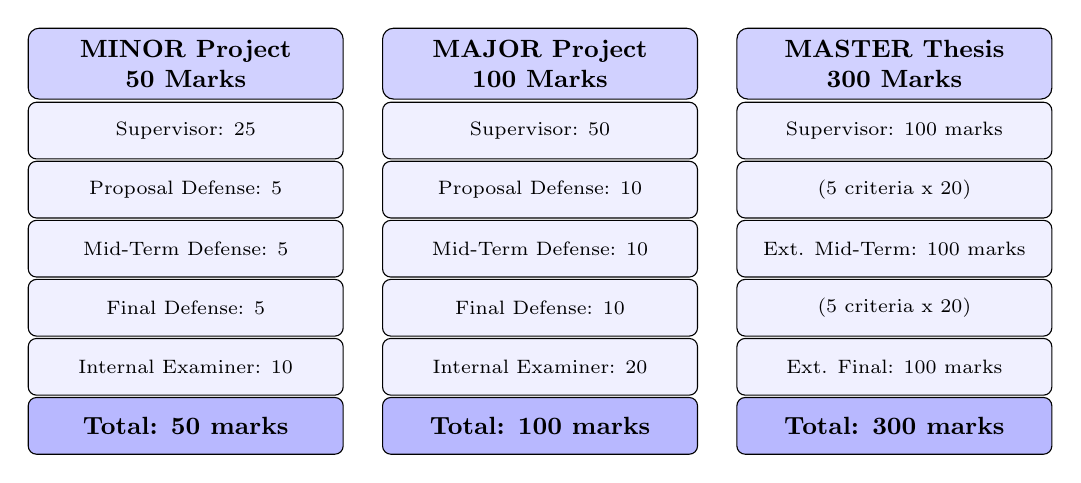
\begin{tikzpicture}[
    hdr/.style={draw, fill=blue!18, rounded corners=4pt, minimum width=4.0cm,
                minimum height=0.9cm, align=center, font=\small\bfseries},
    comp/.style={draw, fill=blue!6, rounded corners=3pt, minimum width=4.0cm,
                 minimum height=0.72cm, align=center, font=\scriptsize},
    tot/.style={draw, fill=blue!28, rounded corners=3pt, minimum width=4.0cm,
                minimum height=0.72cm, align=center, font=\small\bfseries}
]
\node[hdr]  at (-4.5, 6.5) {MINOR Project\\50 Marks};
\node[comp] at (-4.5, 5.65) {Supervisor: 25};
\node[comp] at (-4.5, 4.90) {Proposal Defense: 5};
\node[comp] at (-4.5, 4.15) {Mid-Term Defense: 5};
\node[comp] at (-4.5, 3.40) {Final Defense: 5};
\node[comp] at (-4.5, 2.65) {Internal Examiner: 10};
\node[tot]  at (-4.5, 1.90) {Total: 50 marks};

\node[hdr]  at (0, 6.5) {MAJOR Project\\100 Marks};
\node[comp] at (0, 5.65) {Supervisor: 50};
\node[comp] at (0, 4.90) {Proposal Defense: 10};
\node[comp] at (0, 4.15) {Mid-Term Defense: 10};
\node[comp] at (0, 3.40) {Final Defense: 10};
\node[comp] at (0, 2.65) {Internal Examiner: 20};
\node[tot]  at (0, 1.90) {Total: 100 marks};

\node[hdr]  at (4.5, 6.5) {MASTER Thesis\\300 Marks};
\node[comp] at (4.5, 5.65) {Supervisor: 100 marks};
\node[comp] at (4.5, 4.90) {(5 criteria x 20)};
\node[comp] at (4.5, 4.15) {Ext. Mid-Term: 100 marks};
\node[comp] at (4.5, 3.40) {(5 criteria x 20)};
\node[comp] at (4.5, 2.65) {Ext. Final: 100 marks};
\node[tot]  at (4.5, 1.90) {Total: 300 marks};
\end{tikzpicture}
\caption{TPMS Evaluation Scheme: Mark Distribution by Project Tier}
\label{fig:eval_scheme}
\end{figure}

\subsection{Global Multi-Project Engagement Guard}
Before any group creation, invitation acceptance, or bulk Excel import is committed, the Engagement Guard queries both \texttt{GroupMember} and \texttt{Thesis} tables. If a candidate student is found in ACTIVE or PENDING status, the operation is rejected with a conflict error.

\subsection{Institutional Email Domain Policy}
\begin{itemize}
    \item \textbf{Students:} Email is auto-generated as \texttt{\{rollNumber\}@pcampus.edu.np}.
    \item \textbf{Faculty:} Email must end in \texttt{@pcampus.edu.np}; all other domains are rejected at the API layer.
\end{itemize}
